\part{Multivariate Information Theory }

\section{O-Information}
\begin{frame}[allowframebreaks]{Multimodal Information Theory}
  \begin{itemize}
    \item Recently, the concept of MI has been extended to higher-order interactions: \textbf{{\color{blue} Redundant}, {\color{red} Syngergistic} and {\color{green}Unique}} Information. Seminal works by Williams and Beer (Partial Information Decomposition). Extremely important in consciousness studies.
\begin{figure}
    \centering
   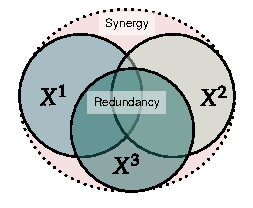
\includegraphics[scale=.7]{figures/info_pdf.pdf}
 \end{figure}
\end{itemize}
\end{frame}
\begin{frame}
Applications: \textbf{Multimodal sensory} Neuroscience studies.
\begin{figure}
    \centering

    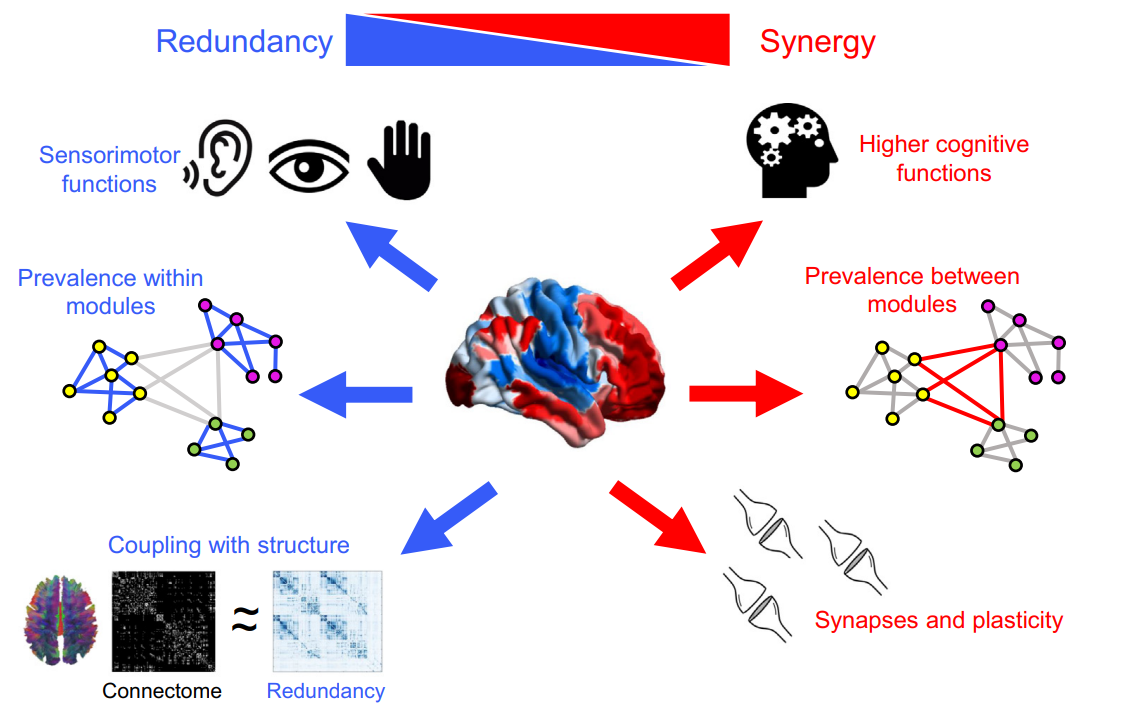
\includegraphics[scale=0.5]{figures/pid_fmri (1).PNG}
   \caption{From Luppi et al, "Information decomposition and the informational architecture of the brain"}
\end{figure}


\end{frame}

\begin{frame}[allowframebreaks]{O-information}
Analyzing systems with more than two variables. Example of metric: \textbf{O-Information}.        
        \begin{itemize}
        \item Mathematically defined as:
        \begin{equation}
            \Omega(X) = T(X) - D(X)
        \end{equation}
        where $T(X) = \sum_{i=1}^{N} H(X_i) - H(X)$ is the Total Correlation and $D(X) = H(X) - \sum_{i=1}^{N} H(X_i | X_{\backslash i})$ is the Dual Total Correlation.
        
        \item Positive O-information indicates redundancy dominance, while negative indicates synergy dominance.
    \end{itemize}
Nice properties, but out of reach unless data Gaussian (or "\textit{simple}") and or discrete. 

\framebreak
Multiple brain regions: is assuming anything a-priori really safe?
\begin{figure}
    \centering
    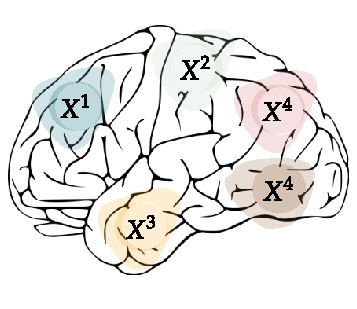
\includegraphics[width=0.5\linewidth]{figures/brain_pdf.pdf}
\end{figure}
We don't need it!!
\end{frame}

\begin{frame}{Score-based (Diffusion) Estimation of O-Information}

    \begin{itemize}
        \item Total Correlation (TC) estimation:
        \begin{equation}
            T(X) = \int p_t(x) \left\| \nabla \log p_t(x) - \sum_{i=1}^{N} \nabla \log p_t(x_i) \right\|^2 dx dt
        \end{equation}
        \item Dual Total Correlation (DTC) estimation:
        \begin{equation}
            D(X) = \int p_t(x) \left\| \nabla \log p_t(x) - \sum_{i=1}^{N} \nabla \log p_t(x_i | x_{\backslash i}) \right\|^2 dx dt
        \end{equation}
        \item with our implementation all the ingredients are \textit{amortized} within a \textit{single} model.
    \end{itemize}
\end{frame}
    



\begin{frame}[allowframebreaks]{Example: Analysis of Mice Brain Activity}
    \begin{itemize}
        \item Study conducted on brain activity of mice brain regions using neural recordings.
         \item Higher O-information in response to new visual stimuli indicates greater redundancy in brain activity.
        \item Lower O-information during repeated stimuli suggests increased synergy.
    \end{itemize}
\begin{figure} [h]
\begin{figure}
    \centering
    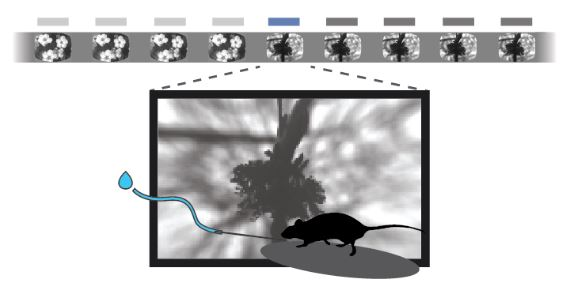
\includegraphics[width=0.5\linewidth]{figures/mouse.JPG}
\end{figure}

\framebreak


\centering
     \begin{subfigure}{0.38\textwidth}
         \centering
         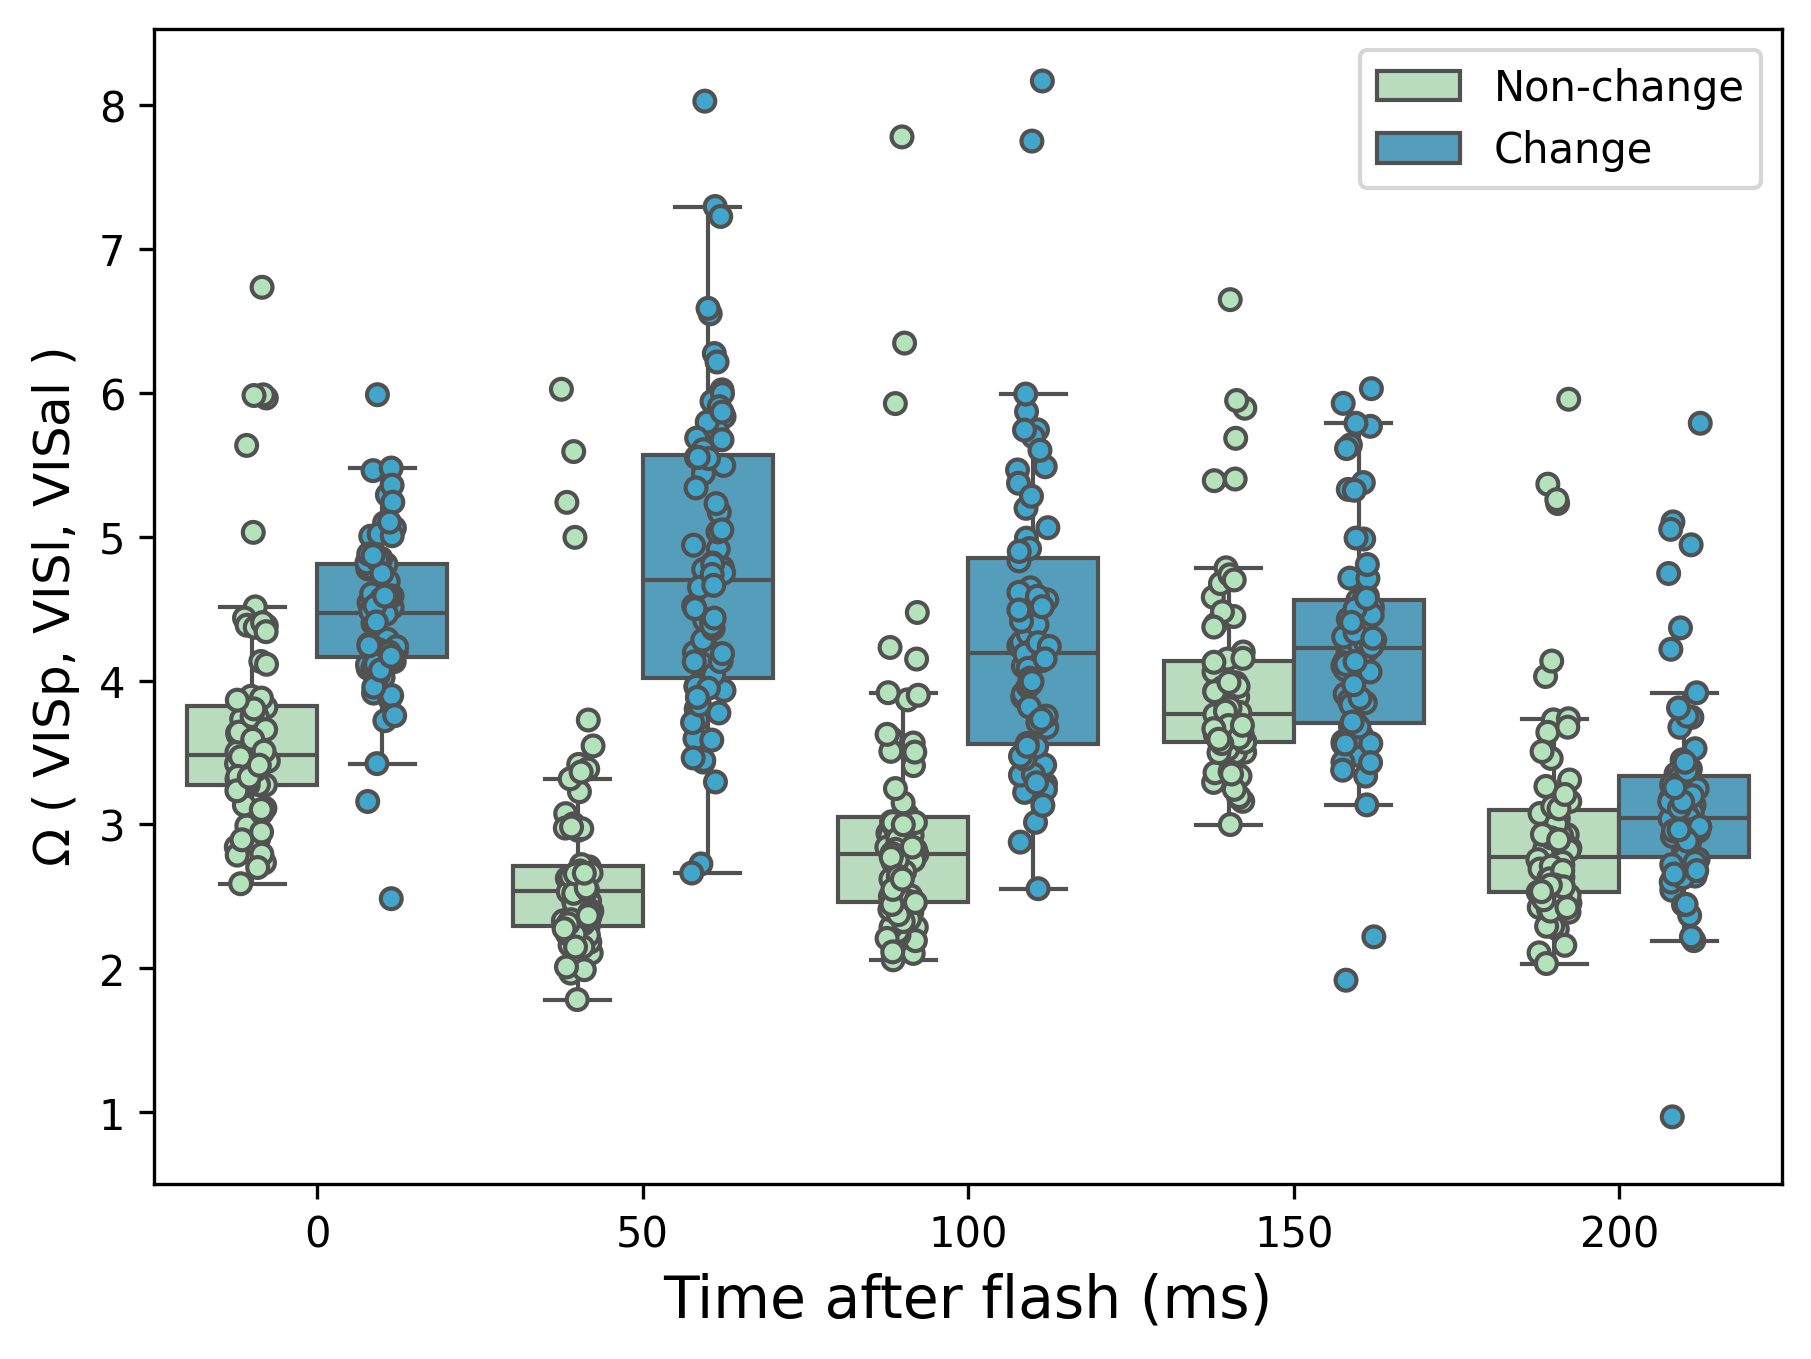
\includegraphics[page=1,width=\linewidth]{figures/new_vbn_setting_3_dim_25.png}
         \caption{3 areas}
     \end{subfigure}
      \begin{subfigure}{0.38\textwidth}
         \centering
         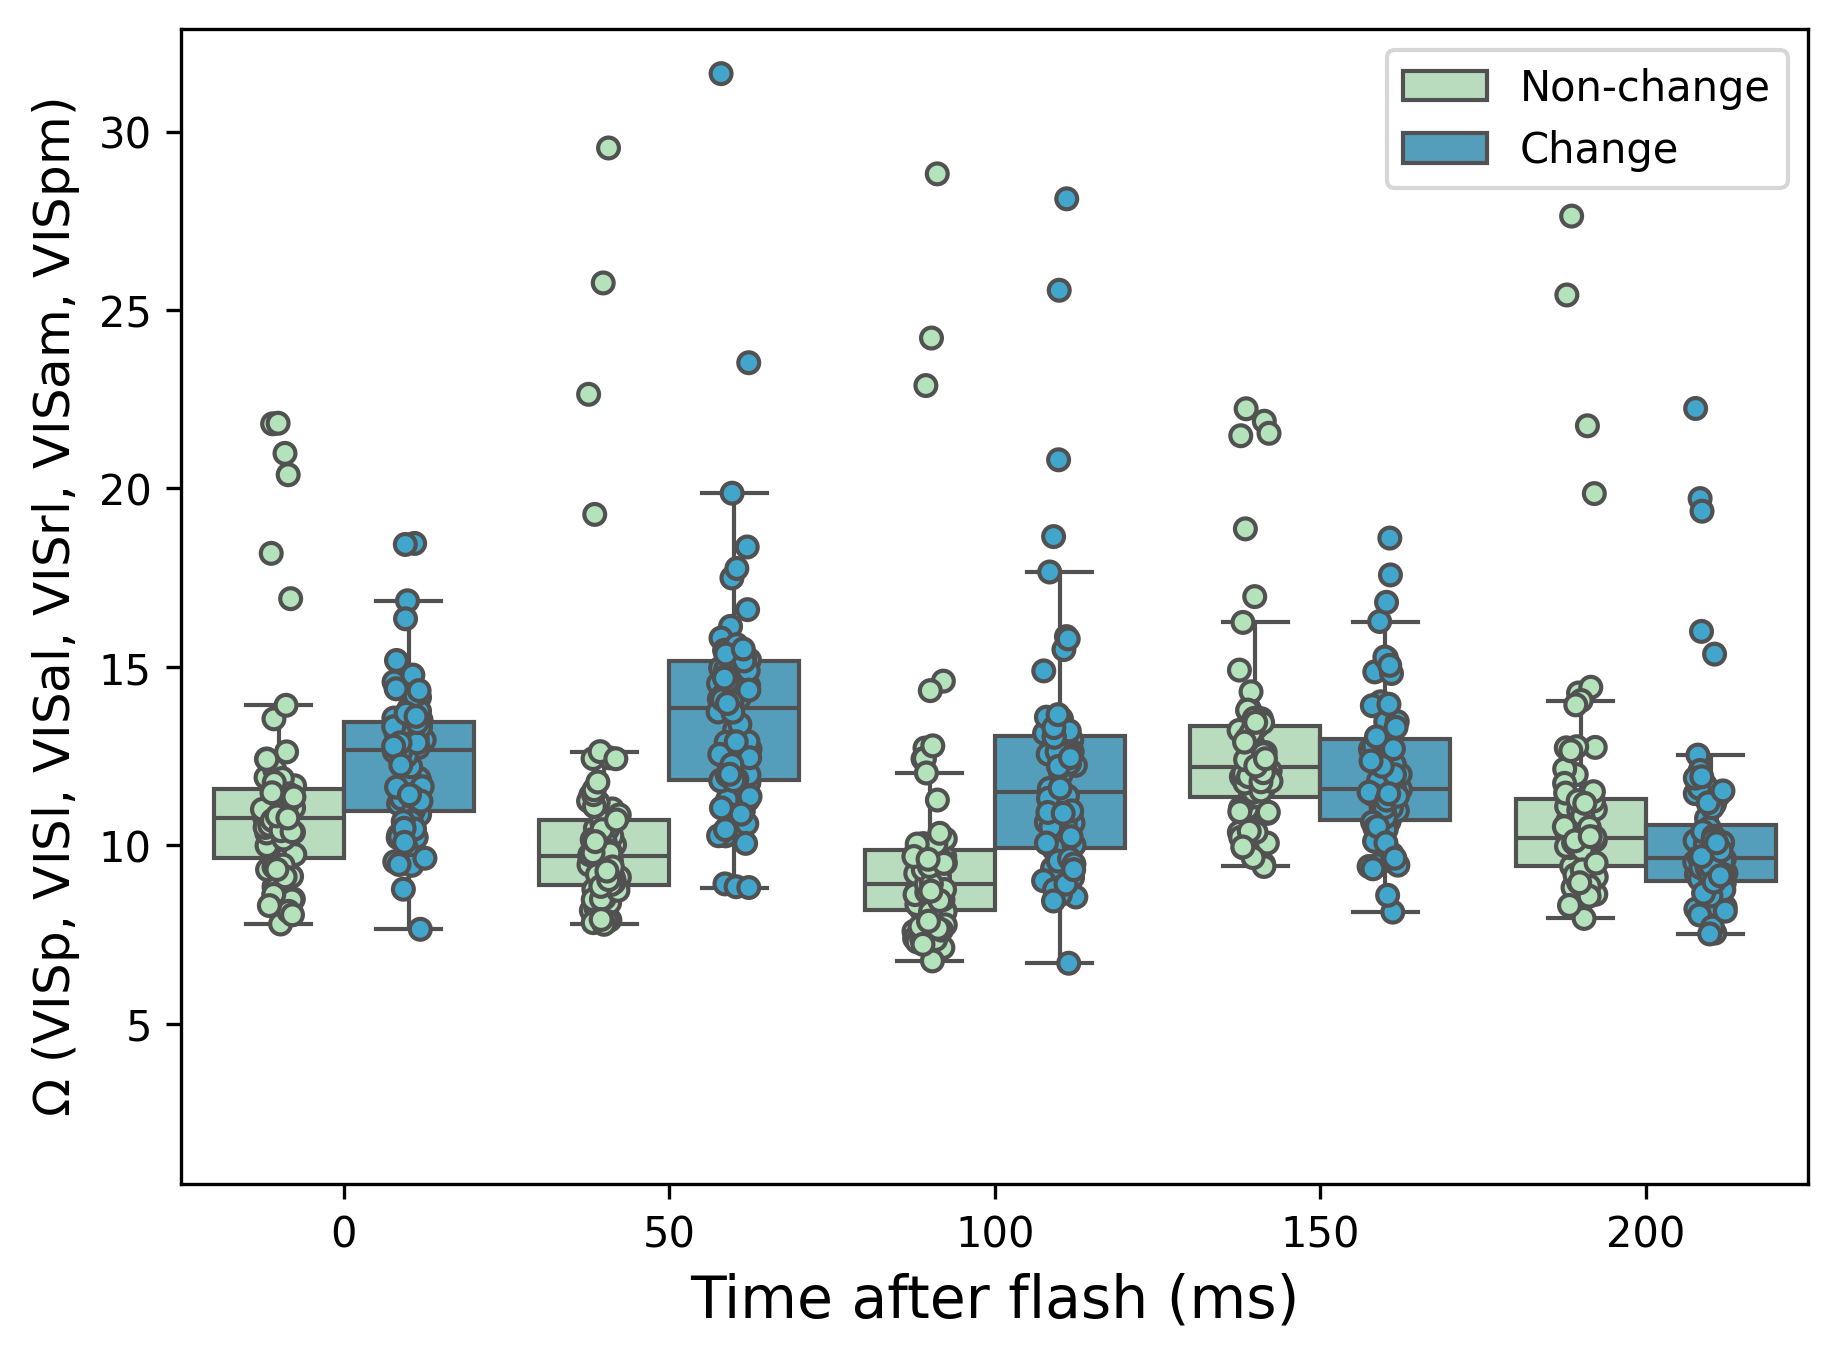
\includegraphics[page=1,width=\linewidth]{figures/new_vbn_setting_6_dim_25.png}
         \caption{6 areas}
     \end{subfigure}

\begin{itemize}
    \item This suggests that higher amount of redundant
information in the visual cortex regions is transmitted in
case of a flash with new scene.
    \item Interestingly, when considering six areas of the visual cortex, our observations remain
valid, suggesting that the measured behaviour is common
to these other brain areas as well.
\end{itemize} 
     
\end{figure}

  
\end{frame}


\section{Transfer Entropy}


\begin{frame}[allowframebreaks]{Temporal Dynamics of Information Metrics}
\begin{itemize}
    \item Transfer entropy measures directed information flow in time series, and it has become
a fundamental quantity in applications spanning neuroscience, finance, and complex systems analysis. 
\item \textit{However} existing estimation
methods suffer from the curse of dimensionality, require restrictive distributional assumptions...
    \item We (work with Simon Pedro Galeano Munoz and Maurizio Filippone - KAUST )  propose
TENDE (Transfer Entropy Neural Diffusion Estimation)
\end{itemize}

\framebreak

\begin{itemize}
    \item Let $\{X_t \}$ and $\{ Y_t \}$ denote discrete time stochastic processes. 
    \item Define 
%
$$
\begin{cases}
\begin{aligned}
\mathbf{Y}_{t-\ell} &= \left[ Y_{t - 1}, \ \dots, \ Y_{t - \ell} \right] \\    
\mathbf{X}_{t-k} &= \left[ X_{t - 1}, \ \dots, \ X_{t - k} \right],
\end{aligned}    
\end{cases}
$$
for some natural numbers $\ell, k $.
\item The TE from $\{X_t \}$ to $\{ Y_t \}$ is given by 
%
\begin{equation}\label{eq:trans_entr}
\mathrm{TE}_{X \to Y}(k,\ell) = I \left ( Y_t; \mathbf{X}_{t - k} \vert \mathbf{Y}_{t - \ell} \right).    
\end{equation}
%
\item TE quantifies how much $Y_t$ depends on the past of $\{X_t\}$ once its past is already known.

\end{itemize}
\framebreak

Example: analysis of asymmetry of information measures in biomedical signals

\begin{figure}
    \centering
    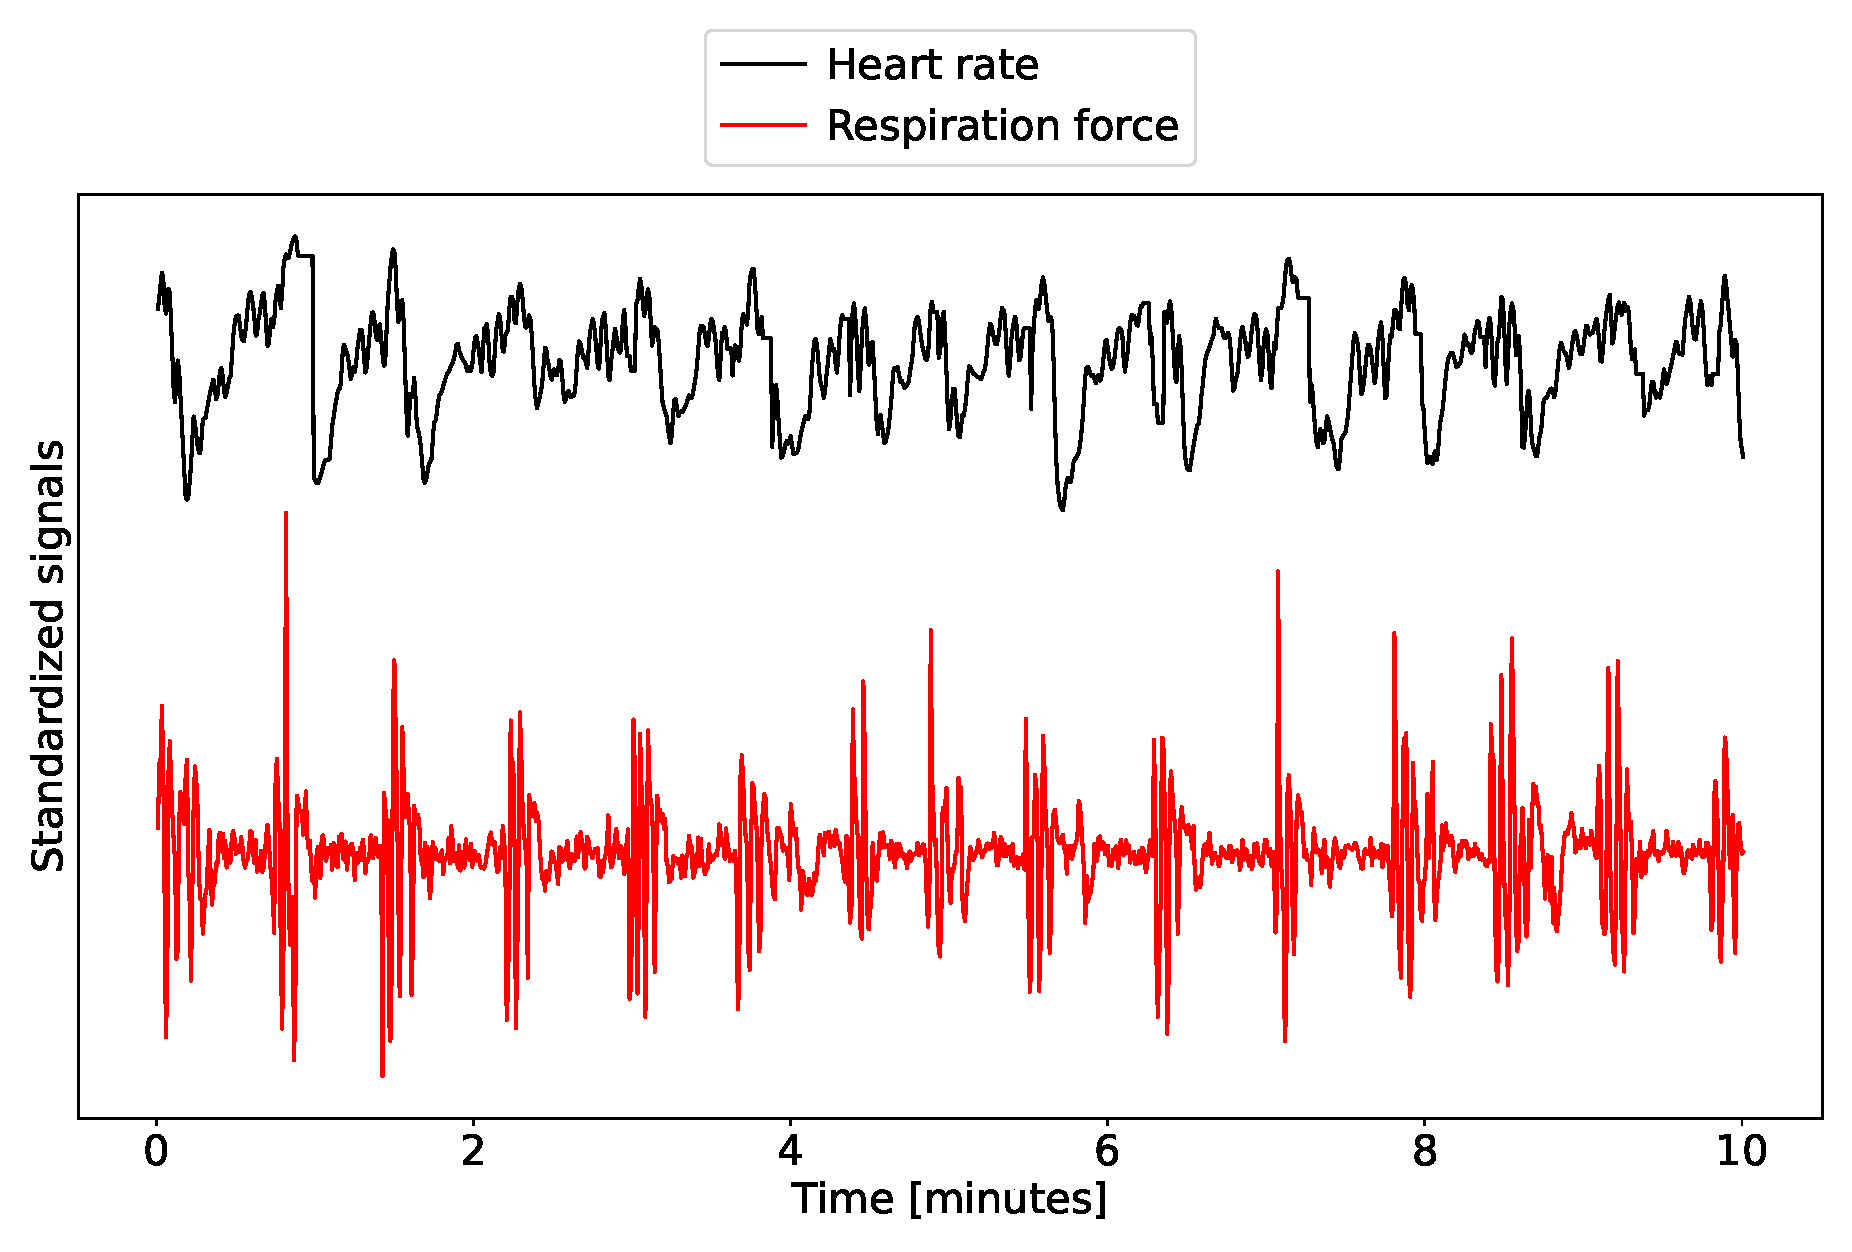
\includegraphics[width=0.5\linewidth]{figures/signals.pdf}
\end{figure}
 \framebreak

\begin{figure}
    \centering
    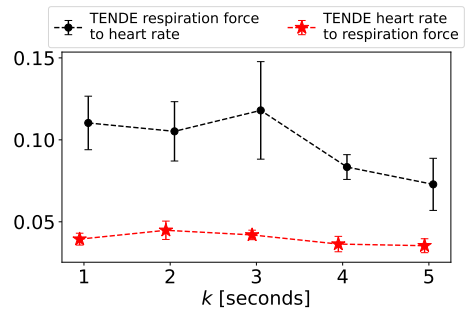
\includegraphics[width=.5\linewidth]{figures/tende_res.PNG}
\end{figure}
\begin{itemize}
    \item TENDE produces stable and physiologically interpretable
estimates.
\item The
declining TE values from respiration to heart rate at
longer lags further indicate that extended cardiac history reduces the incremental predictive contribution of
the breathing signal.
\end{itemize} 
 
\end{frame}
